\documentclass[11pt]{article}

\usepackage[margin=1.1in]{geometry}
\usepackage{times}
\usepackage{amsmath}
\usepackage{booktabs}
\usepackage{graphicx}
\usepackage{natbib}
\usepackage{xcolor}
\usepackage{hyperref}
\usepackage{authblk}
\usepackage{setspace}
\usepackage{microtype}
\usepackage[T1]{fontenc}

\definecolor{linkblue}{RGB}{0,60,140}
\hypersetup{colorlinks=true, linkcolor=linkblue, citecolor=linkblue, urlcolor=linkblue}

\setstretch{1.15}
\setlength{\parskip}{0.4em}
\setlength{\parindent}{0pt}
\setlength{\bibsep}{0.5em}

\title{\textbf{How Often Does a Drift Monitor Cry Wolf?} \\[0.4em] \textbf{Multiple Testing, Reference Sampling, and Autocorrelation in \\ Kolmogorov--Smirnov Monitoring of Sensor Streams}}

\author[1]{Ilahi M. Taofiq\thanks{Corresponding email: taofiqmds24@gmail.com}}
\affil[1]{Independent Research}

\date{}

\begin{document}
\maketitle

\begin{abstract}
Production machine-learning pipelines commonly watch for distribution shift by running a two-sample Kolmogorov--Smirnov (KS) test on every monitored column of each incoming batch against a fixed reference sample, and raising an alarm if any test rejects. We study the false-alarm behaviour and power of this design by simulation, using the column distributions, sample sizes and alarm logic of an open-source industrial-sensor pipeline. First, with three monitored columns and a per-column level of 0.01, the monitor flags 2.9\% of clean batches -- one false alarm every 34 batches on average -- rather than the 1\% the per-column level suggests. Bonferroni, Benjamini--Hochberg and Fisher rules restore a batch-level rate near 1\%; at that size, Bonferroni and Benjamini--Hochberg are most powerful against single-sensor drift, Fisher's rule is most powerful against small simultaneous drift in all sensors, and a ``two of three columns'' rule is nearly blind to single-sensor faults. Second, reusing one fixed reference sample makes false alarms cluster rather than arrive independently: with a 100-row reference, the per-reference false-alarm rate has a standard deviation of 6.9 percentage points, and an alarm is followed by another with probability 20\% versus 2.9\% on average, so requiring two consecutive alarms is far less protective than independence predicts. The reference batch used by the pipeline's own simulation made its pressure column reject 6.8\% of clean batches at a nominal 1\%. Third, autocorrelated sensor readings inflate the KS test's false-alarm rate from 1\% to 17\% at lag-1 autocorrelation 0.6 and 60\% at 0.9; a block-permutation test restores near-nominal size up to autocorrelation 0.6, whereas two simpler remedies, thinning and an effective-sample-size adjustment, respectively lose most of the power or over-correct. Fourth, positive correlation between columns makes Fisher's combination anti-conservative (4.2\% at correlation 0.9). We give concrete, quantified recommendations for reference size, alarm rule and handling of autocorrelation, and release the simulation code and the corrected pipeline.
\end{abstract}

\section{Introduction}

Failures in production machine-learning systems often originate in the data rather than the model: sensors are recalibrated, upstream schemas change, and ambient conditions drift \citep{sculley2015hidden, polyzotis2019validation}. Data-validation and drift-monitoring components are therefore a standard part of ML pipelines \citep{schelter2018deequ, klaise2020monitoring}. A common and simple design tests each monitored feature of every new batch against a fixed reference sample with a two-sample Kolmogorov--Smirnov (KS) test \citep{smirnov1948table, massey1951ks}, using a fixed significance level such as $0.01$ per feature, and raises an alarm if any feature rejects.

This design looks conservative -- a level of $0.01$ suggests a false alarm about once in a hundred batches -- but it rests on three assumptions that are rarely examined. First, \emph{multiplicity}: with $k$ features tested at level $\alpha$ each, the probability that a clean batch triggers at least one rejection is $1-(1-\alpha)^k$, not $\alpha$. Second, \emph{a fixed reference}: the reference sample is drawn once and reused for every later batch, so its own sampling error is shared by every test. If that sample is unrepresentative, every subsequent batch is tested against a slightly wrong yardstick, and false alarms are correlated across batches rather than independent. Third, \emph{independence within a batch}: the KS test assumes independent observations, whereas consecutive sensor readings are typically autocorrelated. Column-to-column correlation additionally affects rules that combine p-values across features.

We quantify all four effects by simulation, on a concrete system: IndustrialFlow, an open-source data and ML pipeline for simulated industrial sensor streams (temperature, vibration, pressure) that validates rows against a schema, scores equipment failure risk, and monitors drift with exactly the design described above. The pipeline's own simulation report documented a false alarm on a clean batch, which motivated this study; as we show in Section~\ref{sec:results}, the explanation originally given for it was incomplete.

\textbf{Contributions.} (1) A quantification of the batch-level false-alarm rate and power of the per-column KS monitor and five alternative alarm rules, compared at equal size. (2) A demonstration that a fixed reference sample makes false alarms cluster, with a measurement of how reference size controls this, and a real instance of the effect in the pipeline's own simulation. (3) A measurement of how autocorrelated readings inflate the KS test's false-alarm rate, and an evaluation of three remedies. (4) A measurement of how column correlation affects each alarm rule. (5) Concrete recommendations and an implementation of the alarm rules in the open-source pipeline.

\section{Background and Related Work}
\label{sec:related}

\textbf{Data validation and monitoring in ML systems.} \citet{sculley2015hidden} identify data dependencies and changes in the external world as major sources of maintenance cost in ML systems. \citet{polyzotis2019validation} describe a data-validation system deployed at scale to detect anomalies in the data fed to production models, and \citet{schelter2018deequ} propose declarative ``unit tests for data'' executed at scale. \citet{klaise2020monitoring} discuss monitoring of deployed models, including outlier and data-drift detection with statistical techniques. Our study is complementary: rather than proposing a new detector, we characterize how often a widely used simple detector raises false alarms and what governs that rate.

\textbf{Dataset shift and drift detection.} Dataset shift is surveyed by \citet{quinonero2009dataset}, and concept drift and its detection by \citet{gama2014survey} and \citet{lu2019learning}. \citet{rabanser2019failing} compare methods for detecting dataset shift and adopt, as a baseline, a two-sample KS test on each dimension aggregated with a Bonferroni correction, which they note is conservative and for which less conservative aggregations exist. We evaluate several such aggregations directly, at equal batch-level size, and study when each is valid.

\textbf{Process-control view.} Monitoring a stream of batches for change is the setting of continuous inspection schemes \citep{page1954continuous}, where the false-alarm behaviour of a scheme is summarized by its in-control average run length, the expected number of batches before a false alarm. We use this framing to translate batch-level rates into operational terms.

\textbf{Multiple testing.} We compare the uncorrected rule with Bonferroni-type corrections \citep{dunn1961multiple}, the Simes/Benjamini--Hochberg procedure \citep{simes1986improved, benjamini1995fdr}, and Fisher's method for combining independent p-values \citep{fisher1932methods}. For the batch-level decision ``was anything rejected?'', Holm's step-down procedure \citep{holm1979simple} coincides with Bonferroni, because its first step is the same test, so we do not evaluate it separately.

\textbf{Dependence and effective sample size.} Autocorrelation reduces the amount of independent information in a sample; \citet{thiebaux1984effective} discuss the resulting effective sample size. We evaluate an effective-sample-size adjustment of the KS test alongside two other remedies in Section~\ref{sec:autocorr}.

\section{Study Design}
\label{sec:design}

\subsection{The monitor under study}

IndustrialFlow validates each incoming batch of about 200 rows against a schema, quarantining invalid rows (about 5\% in its simulation), then compares three monitored columns -- \texttt{temperature\_c}, \texttt{vibration\_mm\_s}, \texttt{pressure\_kpa} -- of the remaining rows against a fixed reference batch using SciPy's two-sample KS test \citep{virtanen2020scipy} (exact p-values at these sample sizes). A column is flagged when $p<\alpha=0.01$, and the batch raises an alarm if any column is flagged; we call this the \emph{uncorrected} rule. Throughout, the reference has $m=285$ and the current batch $n=190$ valid rows, as in the pipeline's own simulation (a 300-row reference and 200-row batches, each with 5\% of rows quarantined).

\subsection{Simulated sensor data}

Each column is drawn from the same marginal distribution the pipeline's data generator uses: temperature $\mathcal N(60,12^2)$~$^\circ$C, vibration $\max(0,\mathcal N(4,1.5^2))$~mm/s, and pressure $\mathcal N(150,20^2)$~kPa. A unit test checks that the simulator's sample means and standard deviations match the pipeline generator's. Drift is a mean shift of a stated number of standard deviations, or a multiplication of the standard deviation. Unless stated, columns and rows are independent.

\subsection{Alarm rules}

Let $p_1,\dots,p_k$ be the per-column KS p-values ($k=3$) and $\alpha=0.01$.
\begin{itemize}
    \item \textbf{Uncorrected} (the released rule): alarm if $\min_i p_i<\alpha$. Under independence its batch-level size is $1-(1-\alpha)^k=2.97\%$.
    \item \textbf{Bonferroni}: alarm if $\min_i p_i<\alpha/k$; size $\le\alpha$.
    \item \textbf{Benjamini--Hochberg (BH)}: alarm if $p_{(i)}\le i\alpha/k$ for some ordered p-value $p_{(i)}$. Used this way it is Simes' test of the global null, with size exactly $\alpha$ for independent p-values.
    \item \textbf{Fisher}: alarm if $-2\sum_i\ln p_i$ exceeds the $1-\alpha$ quantile of $\chi^2_{2k}$; size $\alpha$ for independent p-values.
    \item \textbf{Two of three columns}: alarm if at least two columns each have $p<\alpha_c$. With $\alpha_c=0.01$ its size is $3\alpha_c^2-2\alpha_c^3\approx0.03\%$; we also report a size-calibrated variant with $\alpha_c=0.0589$, chosen so that the size is $1\%$.
\end{itemize}
Bonferroni, BH, Fisher and the calibrated two-of-three rule are all designed for a batch-level size of $1\%$, which lets us compare their power fairly. The uncorrected rule operates at roughly three times that size; higher raw sensitivity at that operating point is not evidence that it is a better detector.

\subsection{Experiments}

\textbf{E1 and E2 (size and power).} For each of eight scenarios (no drift; temperature $+0.25$, $+0.5$, $+1.0$ standard deviations; temperature standard deviation $\times1.5$; all three columns $+0.15$, $+0.25$, $+0.35$ standard deviations) we simulate 10{,}000 independent (reference, batch) pairs with a fresh reference each time, and record how often each rule raises an alarm. A second run varies the batch size with a reference $1.5\times$ larger (5{,}000 replicates per size).

\textbf{E3 (fixed reference).} As in the deployed pipeline, one reference is drawn and reused. For each reference size $m\in\{100,285,1000,5000\}$ we draw 300 references, and test 200 clean batches ($n=190$) against each, recording the alarm sequence per reference. We measure the spread of the false-alarm rate across references, the probability of an alarm given an alarm in the previous batch, the rate of two consecutive alarms compared with the independence prediction, and the share of references with at least one alarm in the first 50 batches. We also run the pipeline's own code path against the reference batch its simulation uses, on 400 clean batches from the pipeline's data generator.

\textbf{E4 (autocorrelation).} Temperature readings follow a stationary AR(1) process with lag-1 autocorrelation $\phi\in\{0,0.3,0.6,0.8,0.9\}$ and unchanged marginal law; the reference and batch are independent contiguous segments. We compare the naive KS test with three remedies, all at nominal level $0.01$ (8{,}000 clean replicates and 3{,}000 replicates per shift): \emph{thinning} both samples by a factor $\lceil(1+\hat\phi)/(1-\hat\phi)\rceil$ (capped at 20) before testing; an \emph{effective-sample-size (ESS) adjustment} that replaces $n$ and $m$ in the asymptotic KS p-value by $n(1-\hat\phi)/(1+\hat\phi)$ and $m(1-\hat\phi)/(1+\hat\phi)$; and a \emph{block-permutation} KS test that shuffles whole blocks of 20 consecutive readings between the two samples (499 permutations), which preserves within-block dependence. Here $\hat\phi$ is the average of the lag-1 sample autocorrelations of the reference and the batch, truncated to $[0,0.98]$.

\textbf{E5 (correlated columns).} The three columns share a Gaussian copula with equal pairwise correlation $\rho\in\{0,0.3,0.6,0.9\}$; rows remain independent. We record the size and the power against a $+0.25$ standard-deviation shift in all columns.

\subsection{Statistical reporting}

Alarm rates are proportions of replicates, reported with 95\% Wilson intervals. All experiments are seeded, and rerunning the released code reproduces every number. Results are simulation results under stated distributions; they describe the behaviour of the alarm logic, not that of any physical plant.

\section{Results}
\label{sec:results}

\subsection{The released monitor flags one clean batch in 34}

Table~\ref{tab:null} shows the batch-level false-alarm rates when the reference is redrawn for every replicate. Each individual column test is valid: the per-column rejection rates are 0.91\%, 0.95\% and 1.04\% against a nominal 1\%. The batch-level rate of the released rule is 2.88\%, matching the theoretical $1-0.99^3=2.97\%$. That is an in-control average run length of about $1/0.0297=34$ batches: with one batch per hour, a false alarm roughly every 34 hours. The Bonferroni, BH, Fisher and calibrated two-of-three rules all sit within sampling error of the intended 1\%, and the two-of-three rule at per-column level 0.01 is extremely conservative (0.02\%).

\begin{table}[htbp]
\centering
\small
\begin{tabular}{lcc}
\toprule
\textbf{Alarm rule} & \textbf{Batches flagged (\%) [95\% CI]} & \textbf{Theory (\%)} \\
\midrule
uncorrected (released) & 2.88 [2.57, 3.23] & 2.97 \\
Bonferroni & 0.97 [0.80, 1.18] & 1.00 \\
Benjamini-Hochberg & 0.97 [0.80, 1.18] & 1.00 \\
Fisher combination & 0.92 [0.75, 1.13] & 1.00 \\
2-of-3 columns (per-column 0.01) & 0.02 [0.01, 0.07] & 0.03 \\
2-of-3 columns (size-calibrated) & 0.91 [0.74, 1.12] & 1.00 \\
\midrule
Single column: temperature c & 0.91 [0.74, 1.12] & 1.00 \\
Single column: vibration mm s & 0.95 [0.78, 1.16] & 1.00 \\
Single column: pressure kpa & 1.04 [0.86, 1.26] & 1.00 \\
\bottomrule
\end{tabular}

\caption{Share of clean batches flagged, with the reference redrawn for every replicate (10{,}000 replicates, $m=285$, $n=190$).}
\label{tab:null}
\end{table}

\subsection{At equal size, the best rule depends on where the drift is}

Figure~\ref{fig:power} and Table~\ref{tab:power} give the share of drifted batches flagged. The uncorrected rule flags the most drifted batches in the single-column scenarios and at the smallest spread-out drift, and is overtaken by Fisher's rule at larger spread-out drift; but it does so at three times the false-alarm rate of the other rules, so its apparent lead is largely a difference of operating point. Among the rules sized at 1\%:
\begin{itemize}
    \item For drift in a \emph{single} sensor, Bonferroni and BH are best: against a $+0.5$ standard-deviation temperature shift they flag 94.9\% of batches, against 89.9\% for Fisher's rule. For single-sensor drift the two are indistinguishable with three columns.
    \item For \emph{small simultaneous} drift in all sensors, Fisher's rule is best: at $+0.25$ standard deviations in every column it flags 81.8\% of batches against 57.0\% for Bonferroni and 58.4\% for BH, and at $+0.15$ it flags 25.9\% against 15.1\% and 15.4\%.
    \item The \emph{two of three columns} rule is structurally unable to detect single-sensor drift: a $+1.0$ standard-deviation temperature shift, which every other rule detects in 100\% of batches, is flagged in only 10.8\% of batches by the size-calibrated version, and only when one of the other two columns happens to cross its threshold by chance. It does detect simultaneous drift (71.5\% at $+0.25$).
\end{itemize}
Table~\ref{tab:powern} shows that detecting a $+0.5$ standard-deviation temperature shift depends strongly on batch size: with 50 rows Bonferroni flags 24.9\% of drifted batches, with 100 rows 62.5\%, with 190 rows 95.0\%.

\begin{figure}[htbp]
\centering
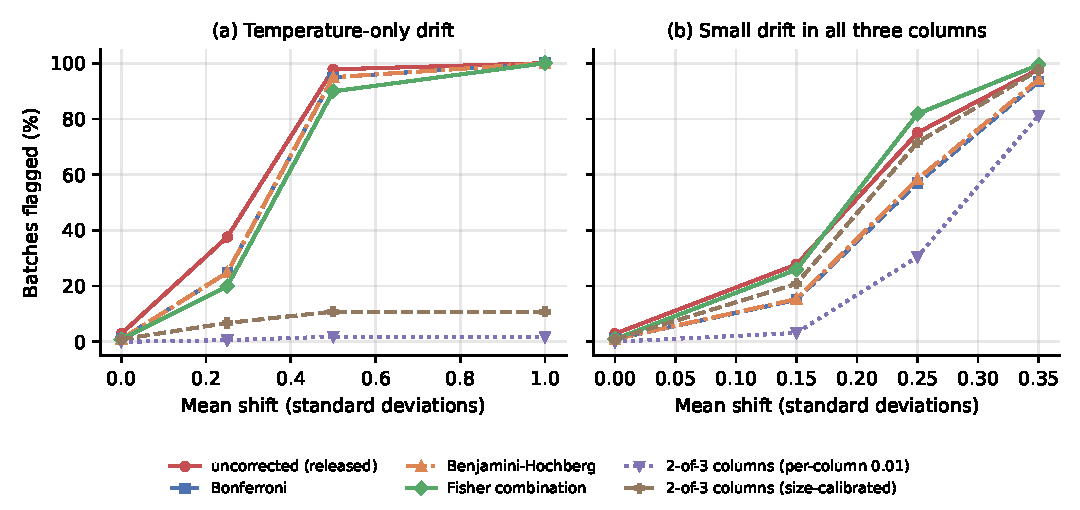
\includegraphics[width=\linewidth]{fig_power.pdf}
\caption{Share of batches flagged as drift grows, by alarm rule. Points at shift 0 are the false-alarm rates. The released (uncorrected) rule runs at roughly three times the size of the others.}
\label{fig:power}
\end{figure}

\begin{table}[htbp]
\centering
\small
\resizebox{\linewidth}{!}{\begin{tabular}{lrrrrrrr}
\toprule
\textbf{Alarm rule} & \textbf{T +0.25} & \textbf{T +0.5} & \textbf{T +1.0} & \textbf{T sd$\times$1.5} & \textbf{All +0.15} & \textbf{All +0.25} & \textbf{All +0.35} \\
\midrule
uncorrected (released) & 37.6 & 97.8 & 100.0 & 36.3 & 27.8 & 75.0 & 97.8 \\
Bonferroni & 24.9 & 94.9 & 100.0 & 19.4 & 15.1 & 57.0 & 93.3 \\
Benjamini-Hochberg & 24.9 & 95.0 & 100.0 & 19.5 & 15.3 & 58.4 & 94.1 \\
Fisher combination & 19.9 & 89.9 & 100.0 & 15.4 & 25.9 & 81.8 & 99.4 \\
2-of-3 columns (per-column 0.01) & 0.6 & 1.8 & 1.7 & 0.7 & 3.2 & 30.5 & 81.2 \\
2-of-3 columns (size-calibrated) & 6.8 & 10.8 & 10.8 & 8.2 & 20.8 & 71.5 & 97.5 \\
\bottomrule
\end{tabular}
}
\caption{Batches flagged (\%) by drift scenario. T = temperature only; All = all three columns; shifts in standard deviations.}
\label{tab:power}
\end{table}

\begin{table}[htbp]
\centering
\small
\resizebox{\linewidth}{!}{\begin{tabular}{rrrrr}
\toprule
\textbf{Batch rows} & \textbf{Ref.\ rows} & \textbf{uncorrected (released)} & \textbf{Bonferroni} & \textbf{Fisher combination} \\
\midrule
50 & 75 & 41.3 & 24.9 & 20.2 \\
100 & 150 & 75.8 & 62.5 & 52.5 \\
190 & 285 & 98.1 & 95.0 & 90.4 \\
500 & 750 & 100.0 & 100.0 & 100.0 \\
\bottomrule
\end{tabular}
}
\caption{Batches flagged (\%) against a $+0.5$ standard-deviation temperature shift, by batch size.}
\label{tab:powern}
\end{table}

\subsection{A fixed reference makes false alarms cluster}
\label{sec:reference}

The averages above assume a fresh reference for every batch. A deployed monitor reuses one. Averaged over reference draws, the false-alarm rate stays at its nominal value (2.5--2.9\% for the released rule in Table~\ref{tab:reference}), but the rate \emph{for a given reference} varies enormously when the reference is small. With 100 reference rows, the per-reference rate has a standard deviation of 6.9 percentage points and the worst of 300 references raised an alarm on 64.5\% of clean batches; 40\% of references never alarmed in 200 batches, and 13\% had a rate more than twice the average. (With only 200 batches per reference, sampling noise alone would give a standard deviation near 1.2 points; the excess is reference-to-reference variation, and it vanishes by $m=5000$.) With the released size, $m=285$, the standard deviation is 3.1 points, the 95th-percentile reference has a rate of 8.0\% and the worst 26\%.

\begin{figure}[htbp]
\centering
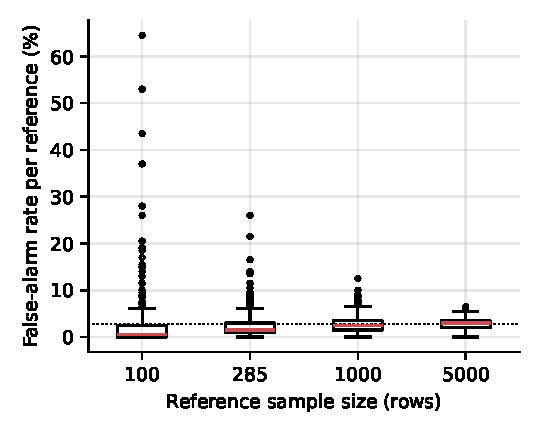
\includegraphics[width=0.55\linewidth]{fig_reference.pdf}
\caption{False-alarm rate of the released rule for each of 300 fixed references (200 clean batches each), by reference size. Dotted line: mean across all.}
\label{fig:reference}
\end{figure}

\begin{table}[htbp]
\centering
\small
\resizebox{\linewidth}{!}{\begin{tabular}{rrrrrrr}
\toprule
\textbf{Ref.\ rows} & \textbf{Mean (\%)} & \textbf{SD (\%)} & \textbf{$>2\times$ mean} & \textbf{P(alarm$\mid$prev.)} & \textbf{$\geq$1 in 50} & \textbf{if indep.} \\
\midrule
100 & 2.87 & 6.90 & 13\% & 20.4\% & 35\% & 77\% \\
285 & 2.52 & 3.07 & 11\% & 5.9\% & 60\% & 72\% \\
1000 & 2.88 & 1.78 & 6\% & 3.8\% & 72\% & 77\% \\
5000 & 2.89 & 1.16 & 1\% & 3.0\% & 77\% & 77\% \\
\bottomrule
\end{tabular}
}
\caption{Released (uncorrected) rule with a fixed reference: mean and standard deviation of the per-reference false-alarm rate; share of references whose rate exceeds twice the mean; probability of an alarm given an alarm in the previous batch; share of references with at least one alarm in the first 50 batches, and the value independence would predict.}
\label{tab:reference}
\end{table}

The consequence is that alarms arrive in bursts. With $m=100$, the probability of an alarm immediately after an alarm is 20.4\% against a 2.9\% average, and the rate of two consecutive alarms is 0.59\% against 0.08\% if alarms were independent (a factor of 7). At $m=285$ the factors are 5.9\% against 2.5\% and 0.15\% against 0.06\% (2.3$\times$). Bonferroni and Fisher show the same pattern (at $m=100$, an alarm is followed by another with probability 15\% for both, against average rates near 1\%). This matters in practice because a common mitigation for alert fatigue is to \emph{require two consecutive alarms}: under independence that would cut the false-alarm rate by a factor equal to the inverse of the single-batch alarm rate (about 34 here), but with a small reference it removes far less than that, since the batches most likely to alarm are concentrated in the references that alarm often. Larger references restore near-independence: at $m=1000$ the two-consecutive rate exceeds the independence value by a factor of 1.3, and at $m=5000$ it is close to it (0.087\% against 0.083\%).

\textbf{A real instance.} The pipeline's own simulation reuses one 300-row reference (285 valid rows). Running the pipeline's real code path against it on 400 clean batches from the real data generator, the pressure column rejects 27 times (6.75\%, 95\% CI 4.7--9.6\%), against a nominal 1\%, while temperature (1.0\%) and vibration (0.25\%) are close to or below nominal. The released rule therefore flags 8.0\% of clean batches (CI 5.7--11.1\%) instead of 2.97\%, and even the Bonferroni, BH and Fisher rules flag 3.0\% (CI 1.7--5.2\%) instead of 1\%. The single false alarm in the pipeline's simulation report (batch \texttt{normal\_6}, with a pressure p-value of 0.0004) had originally been attributed to uncorrected multiple testing. Multiple testing does raise the rate, by about a factor of three, but this reference batch, which is unrepresentative for pressure, raises it by a further factor of about 2.7 for the released rule (8.0\% against 2.97\%) and about 3 for the corrected rules (3.0\% against 1\%). No alarm rule fixes the second effect; only a larger or better-validated reference does.

\subsection{Autocorrelated readings}
\label{sec:autocorr}

Table~\ref{tab:autocorr} and Figure~\ref{fig:autocorr} show the effect of autocorrelation on the temperature column. The naive KS test's false-alarm rate, nominally 1\%, is 0.96\% for independent readings and grows to 3.96\% at lag-1 autocorrelation $\phi=0.3$, 16.7\% at $\phi=0.6$, 37.4\% at $\phi=0.8$ and 60.0\% at $\phi=0.9$. Autocorrelated observations carry less independent information than their number suggests, so the empirical distribution functions fluctuate more than the independent-sample null distribution allows. The naive test's apparent power at high $\phi$ (79.8\% against a $+0.5$ standard-deviation shift at $\phi=0.9$) is therefore not sensitivity: at that autocorrelation a batch with no drift at all is flagged 60\% of the time.

\begin{figure}[htbp]
\centering
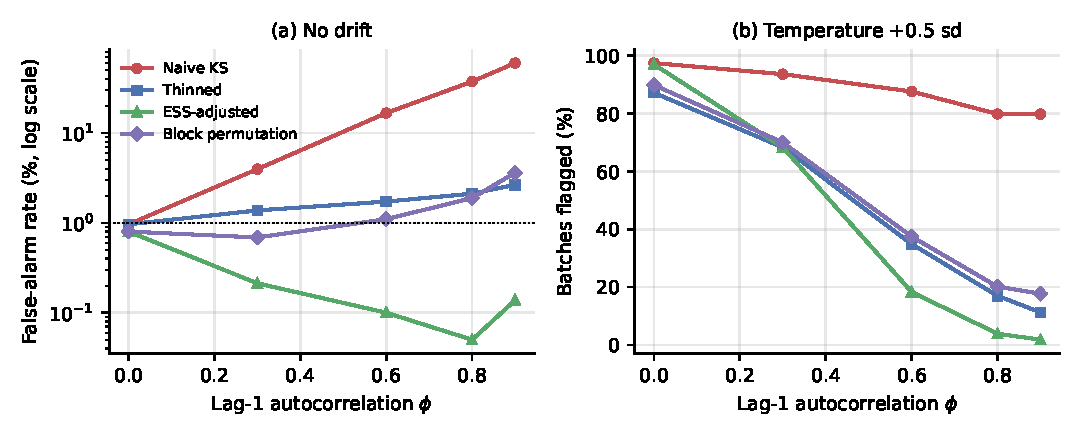
\includegraphics[width=\linewidth]{fig_autocorr.pdf}
\caption{Effect of lag-1 autocorrelation on the KS drift test, with three remedies. (a) False-alarm rate on clean batches (log scale; dotted line is the nominal 1\%). (b) Share of batches flagged against a $+0.5$ standard-deviation shift.}
\label{fig:autocorr}
\end{figure}

\begin{table}[htbp]
\centering
\small
\begin{tabular}{rcccc@{\hspace{1.6em}}cccc}
\toprule
 & \multicolumn{4}{c}{\textbf{No drift: flagged (\%)}} & \multicolumn{4}{c}{\textbf{Temperature +0.5 sd: flagged (\%)}} \\
\cmidrule(lr){2-5}\cmidrule(lr){6-9}
$\phi$ & Naive & Thin & ESS & Block & Naive & Thin & ESS & Block \\
\midrule
0.0 & 0.96 & 0.96 & 0.80 & 0.80 & 97.5 & 87.2 & 97.0 & 89.9 \\
0.3 & 3.96 & 1.38 & 0.21 & 0.69 & 93.6 & 68.3 & 68.3 & 70.0 \\
0.6 & 16.68 & 1.73 & 0.10 & 1.10 & 87.6 & 34.9 & 18.3 & 37.5 \\
0.8 & 37.40 & 2.11 & 0.05 & 1.89 & 79.9 & 17.0 & 3.9 & 20.1 \\
0.9 & 60.02 & 2.65 & 0.14 & 3.61 & 79.8 & 11.2 & 1.8 & 17.7 \\
\bottomrule
\end{tabular}

\caption{Batches flagged (\%) by autocorrelation $\phi$ and method: the naive KS test; thinning by the estimated autocorrelation; the effective-sample-size (ESS) adjustment; and the block-permutation test (blocks of 20 rows, 499 permutations). All at nominal level 0.01.}
\label{tab:autocorr}
\end{table}

The three remedies behave very differently.
\begin{itemize}
    \item \textbf{Thinning} keeps the size close to nominal (1.4\% at $\phi=0.3$ up to 2.7\% at $\phi=0.9$), at a large cost in power: the flag rate against the $+0.5$ standard-deviation shift falls from 87.2\% at $\phi=0$ to 34.9\% at $\phi=0.6$ and 11.2\% at $\phi=0.9$.
    \item The \textbf{ESS adjustment} over-corrects badly. Its size is 0.05--0.2\% for $\phi\ge0.3$, far below nominal, and its power collapses (18.3\% at $\phi=0.6$, 1.8\% at $\phi=0.9$). We conjecture that the factor $(1-\phi)/(1+\phi)$, which is the variance inflation of the sample \emph{mean} of an AR(1) process, overstates the dependence of the indicator functions from which an empirical distribution function is built; we did not test this explanation.
    \item The \textbf{block-permutation test} is the best of the three. Its size is 0.69--1.10\% for $\phi\le0.6$, 1.89\% at $\phi=0.8$ and 3.61\% at $\phi=0.9$ (95\% CI 3.2--4.0\%); the residual inflation at high $\phi$ is expected, since the 20-row blocks are not long relative to the correlation length (the lag-20 autocorrelation is 0.01 at $\phi=0.8$ but 0.12 at $\phi=0.9$, so neighbouring blocks remain dependent). Its power is at or above thinning's at every $\phi\ge0.3$ (37.5\% against 34.9\% at $\phi=0.6$, 20.1\% against 17.0\% at $\phi=0.8$), though at $\phi=0.9$ this comparison is at a somewhat larger size (3.6\% against 2.7\%).
\end{itemize}
No remedy keeps high power under strong autocorrelation, and that is an information limit rather than a defect of any test: at $\phi=0.8$ a 190-row batch contains the equivalent of roughly $190\times(1-\phi)/(1+\phi)\approx21$ independent observations. Detecting small shifts in strongly autocorrelated signals requires longer batches or a lower sampling rate, not a cleverer test.

\subsection{Correlated sensor columns}

Real sensor columns are rarely independent. Table~\ref{tab:correlated} shows the effect of positive correlation between columns. The uncorrected rule, Bonferroni and BH become more conservative as correlation grows (at $\rho=0.9$ the uncorrected rule flags 2.0\% of clean batches, Bonferroni 0.72\% and BH 0.79\%), because correlated tests reject together and the union of rejections shrinks. Fisher's combination goes the other way: its false-alarm rate rises from 0.90\% at $\rho=0$ to 1.15\%, 2.43\% and 4.19\% at $\rho=0.3$, $0.6$ and $0.9$, since the method assumes independent p-values. The calibrated two-of-three rule inflates similarly (3.92\% at $\rho=0.9$). Fisher's power advantage on simultaneous drift persists (68.2\% against 38.4\% for Bonferroni at $\rho=0.9$) but part of it is bought with a 4$\times$ inflated size, so it should not be read as a clean win when columns are strongly correlated.

\begin{table}[htbp]
\centering
\small
\resizebox{\linewidth}{!}{\begin{tabular}{lrrrr@{\hspace{1.6em}}rrrr}
\toprule
 & \multicolumn{4}{c}{\textbf{No drift: flagged (\%)}} & \multicolumn{4}{c}{\textbf{All columns +0.25 sd: flagged (\%)}} \\
\cmidrule(lr){2-5}\cmidrule(lr){6-9}
\textbf{Alarm rule} & $\rho{=}0.0$ & $\rho{=}0.3$ & $\rho{=}0.6$ & $\rho{=}0.9$ & $\rho{=}0.0$ & $\rho{=}0.3$ & $\rho{=}0.6$ & $\rho{=}0.9$ \\
\midrule
uncorrected (released) & 2.88 & 2.58 & 2.53 & 2.00 & 75.2 & 68.8 & 63.2 & 52.6 \\
Bonferroni & 1.02 & 1.00 & 0.86 & 0.72 & 58.0 & 51.9 & 47.3 & 38.4 \\
Benjamini-Hochberg & 1.03 & 1.00 & 0.88 & 0.79 & 59.3 & 53.1 & 48.6 & 40.1 \\
Fisher combination & 0.90 & 1.15 & 2.43 & 4.19 & 82.4 & 75.8 & 72.9 & 68.2 \\
2-of-3 columns (per-column 0.01) & 0.01 & 0.02 & 0.16 & 0.57 & 31.1 & 33.3 & 34.8 & 36.2 \\
2-of-3 columns (size-calibrated) & 0.67 & 1.00 & 2.29 & 3.92 & 71.6 & 68.9 & 67.7 & 65.9 \\
\bottomrule
\end{tabular}
}
\caption{Batches flagged (\%) when the three columns are correlated (equal pairwise correlation $\rho$), with no drift and with a $+0.25$ standard-deviation shift in every column.}
\label{tab:correlated}
\end{table}

\section{Discussion and Recommendations}

The four effects above translate into concrete choices for a KS-based monitor.

\textbf{State the batch-level false-alarm budget, then derive the per-column level.} A per-column level is not an alarm rate. Choosing a target in-control run length (say one false alarm per 1000 batches, a batch-level size of $0.1\%$) and applying a Bonferroni or BH rule at that level is a one-line change; the released pipeline now exposes the rule as a parameter (\texttt{drift\_rule}), leaving the historical behaviour as default.

\textbf{Choose the rule by the expected failure mode.} If isolated sensor faults are the main concern, use Bonferroni or BH. If small, diffuse changes across many sensors matter, Fisher's rule detects them sooner, but only when columns are weakly correlated; with strongly correlated columns its threshold must be calibrated (for example by permutation) or the inflated false-alarm rate accepted. Rules that require several columns to agree should be avoided unless single-sensor faults are out of scope.

\textbf{Make the reference large, and audit it.} A reference of a few hundred rows is enough for a valid test on average but not for a predictable alarm rate. In our simulation the reference-to-reference standard deviation of the false-alarm rate falls from 6.9 points at 100 rows to 1.8 at 1000 and to the sampling-noise floor at 5000. Independently of size, a reference can be checked before deployment by running the monitor on held-out clean data and confirming the alarm rate is near its target: the pipeline's simulation reference would have failed such a check (8.0\% against 2.97\%).

\textbf{Do not count on consecutive-alarm rules with a small reference.} They are much less protective than independence suggests.

\textbf{Measure autocorrelation before trusting a KS test.} The lag-1 autocorrelation of each monitored column in the reference is cheap to compute. Above roughly $0.3$ the naive test's false-alarm rate is already several times nominal, and above $0.6$ it is unusable. In our simulation a block-permutation test kept the size near nominal up to $\phi=0.6$ and within a factor of four of it up to $\phi=0.9$; block length should be long relative to the correlation length. If autocorrelation is strong, longer batches or a lower sampling rate are the only way to recover sensitivity.

\section{Limitations}

All results are from simulations with Gaussian marginals, a stationary reference and stationary clean batches; real sensor data have heavier tails, seasonality and slow trends, and the study says nothing about how an alarm relates to model performance degradation. Drift is modelled as a step change in mean or variance, not gradual drift or change points. Only the two-sample KS test is studied, not other detectors, and the columns are three in number, so the multiplicity effects would be larger with more monitored features. Column dependence is modelled by a Gaussian copula with equal correlations and the temporal dependence by an AR(1) process; other structures could behave differently. Batch sizes and reference sizes are those of one pipeline. The simulations sample independent references and batches and therefore do not capture data-dependent feedback, such as a reference refreshed from recent batches. Finally, the pipeline and the simulator are written by the same author; the released code and seeds are provided so that the results can be checked independently.

\section{Reproducibility and Code Availability}

The pipeline, the simulation code (\texttt{src/industrialflow/drift\_study.py}), the figure and table generator, the raw result files and a test suite are available at \url{https://github.com/taofiq23/IndustrialFlow}. Every experiment is seeded; the released results were produced with NumPy and SciPy (versions recorded in each result file). The complete study runs in under an hour on a single CPU core.

\section{Conclusion}

A per-column KS monitor with a fixed level looks safe but raises false alarms about three times more often than its level suggests when three columns are tested; reusing a small fixed reference makes those false alarms bursty; autocorrelation in the readings can inflate them by more than an order of magnitude; and correlated columns break the most powerful combination rule. Each of these can be measured cheaply before deployment, and each has a straightforward mitigation. We hope the quantified recommendations, and the released code that reproduces them, are useful to teams operating drift monitors on sensor data.

\bibliographystyle{plainnat}
\begin{thebibliography}{18}

\bibitem[Benjamini and Hochberg(1995)]{benjamini1995fdr}
Yoav Benjamini and Yosef Hochberg.
\newblock Controlling the false discovery rate: a practical and powerful approach to multiple testing.
\newblock \emph{Journal of the Royal Statistical Society: Series B}, 57(1):289--300, 1995.

\bibitem[Dunn(1961)]{dunn1961multiple}
Olive Jean Dunn.
\newblock Multiple comparisons among means.
\newblock \emph{Journal of the American Statistical Association}, 56(293):52--64, 1961.

\bibitem[Fisher(1932)]{fisher1932methods}
Ronald A. Fisher.
\newblock \emph{Statistical Methods for Research Workers}.
\newblock Oliver and Boyd, Edinburgh, 4th edition, 1932.

\bibitem[Gama et al.(2014)]{gama2014survey}
Jo{\~a}o Gama, Indr{\.e} {\v{Z}}liobait{\.e}, Albert Bifet, Mykola Pechenizkiy, and Abdelhamid Bouchachia.
\newblock A survey on concept drift adaptation.
\newblock \emph{ACM Computing Surveys}, 46(4):Article 44, 2014.

\bibitem[Holm(1979)]{holm1979simple}
Sture Holm.
\newblock A simple sequentially rejective multiple test procedure.
\newblock \emph{Scandinavian Journal of Statistics}, 6(2):65--70, 1979.

\bibitem[Klaise et al.(2020)]{klaise2020monitoring}
Janis Klaise, Arnaud Van Looveren, Clive Cox, Giovanni Vacanti, and Alexandru Coca.
\newblock Monitoring and explainability of models in production.
\newblock \emph{arXiv preprint arXiv:2007.06299}, 2020.

\bibitem[Lu et al.(2019)]{lu2019learning}
Jie Lu, Anjin Liu, Fan Dong, Feng Gu, Jo{\~a}o Gama, and Guangquan Zhang.
\newblock Learning under concept drift: a review.
\newblock \emph{IEEE Transactions on Knowledge and Data Engineering}, 31(12):2346--2363, 2019.

\bibitem[Massey(1951)]{massey1951ks}
Frank J. Massey, Jr.
\newblock The Kolmogorov--Smirnov test for goodness of fit.
\newblock \emph{Journal of the American Statistical Association}, 46(253):68--78, 1951.

\bibitem[Page(1954)]{page1954continuous}
E. S. Page.
\newblock Continuous inspection schemes.
\newblock \emph{Biometrika}, 41(1--2):100--115, 1954.

\bibitem[Polyzotis et al.(2019)]{polyzotis2019validation}
Neoklis Polyzotis, Martin Zinkevich, Sudip Roy, Eric Breck, and Steven Whang.
\newblock Data validation for machine learning.
\newblock In \emph{Proceedings of Machine Learning and Systems (MLSys)}, volume 1, 2019.

\bibitem[Qui{\~n}onero-Candela et al.(2009)]{quinonero2009dataset}
Joaquin Qui{\~n}onero-Candela, Masashi Sugiyama, Anton Schwaighofer, and Neil D. Lawrence, editors.
\newblock \emph{Dataset Shift in Machine Learning}.
\newblock MIT Press, 2009.

\bibitem[Rabanser et al.(2019)]{rabanser2019failing}
Stephan Rabanser, Stephan G{\"u}nnemann, and Zachary C. Lipton.
\newblock Failing loudly: an empirical study of methods for detecting dataset shift.
\newblock In \emph{Advances in Neural Information Processing Systems (NeurIPS)}, volume 32, 2019.

\bibitem[Schelter et al.(2018)]{schelter2018deequ}
Sebastian Schelter, Dustin Lange, Philipp Schmidt, Meltem Celikel, Felix Bie{\ss}mann, and Andreas Grafberger.
\newblock Automating large-scale data quality verification.
\newblock \emph{Proceedings of the VLDB Endowment}, 11(12):1781--1794, 2018.

\bibitem[Sculley et al.(2015)]{sculley2015hidden}
D. Sculley, Gary Holt, Daniel Golovin, Eugene Davydov, Todd Phillips, Dietmar Ebner, Vinay Chaudhary, Michael Young, Jean-Fran{\c{c}}ois Crespo, and Dan Dennison.
\newblock Hidden technical debt in machine learning systems.
\newblock In \emph{Advances in Neural Information Processing Systems (NeurIPS)}, volume 28, pages 2503--2511, 2015.

\bibitem[Simes(1986)]{simes1986improved}
R. J. Simes.
\newblock An improved Bonferroni procedure for multiple tests of significance.
\newblock \emph{Biometrika}, 73(3):751--754, 1986.

\bibitem[Smirnov(1948)]{smirnov1948table}
N. V. Smirnov.
\newblock Table for estimating the goodness of fit of empirical distributions.
\newblock \emph{Annals of Mathematical Statistics}, 19(2):279--281, 1948.

\bibitem[Thi{\'e}baux and Zwiers(1984)]{thiebaux1984effective}
Jean H. Thi{\'e}baux and Francis W. Zwiers.
\newblock The interpretation and estimation of effective sample size.
\newblock \emph{Journal of Climate and Applied Meteorology}, 23(5):800--811, 1984.

\bibitem[Virtanen et al.(2020)]{virtanen2020scipy}
Pauli Virtanen, Ralf Gommers, Travis E. Oliphant, et al.
\newblock {SciPy} 1.0: fundamental algorithms for scientific computing in {Python}.
\newblock \emph{Nature Methods}, 17(3):261--272, 2020.

\end{thebibliography}

\end{document}
